\subsection{Overview}

Once we have produced this synthetic travel demand data, we model the regional circulation network for traffic assignment. Our integrated pipeline models networks as mathematical graphs consisting of a set of nodes \textit{N} connected to one another by a set of edges \textit{E} \citep{newman_networks:_2010,gastner_spatial_2006}. Specifically, the road network is modeled as a nonplanar directed multigraph with possible self-loops. The data come from OpenStreetMap.

This section describes how we acquire these data, construct a graph model of the network, process its topology, and calculate and impute relevant variables. Next it describes the process of calculating BPR coefficients and the assumptions baked into this calculation. Finally, it explains the process of converting the zone-based travel demand output from ActivitySim to a network node-based demand data set. 

\subsection{Network creation, construction, and processing}

The network data in this modeling pipeline come from OpenStreetMap. OpenStreetMap is a public worldwide collaborative mapping project and web platform with over two million users. Anyone may edit or access OpenStreetMap data, but community oversight and standards exist to prevent significant vandalism or inaccurate edits \citep{jokar_arsanjani_openstreetmap_2015}. In general, OpenStreetMap data are of high accuracy and quality, particularly in the United States and Western Europe \citep{corcoran_analysing_2013,over_generating_2010,haklay_how_2010,maron_how_2015}. OpenStreetMap imported the 2005 TIGER/Line roads data set as a foundation, and numerous corrections and additions to these data have been made since \citep{willis_openstreetmap_2008}.

The network graph is constructed using OSMnx, an open-source Python package for working with OpenStreetMap data \citep{boeing_osmnx:_2017}. OSMnx is built on top of NetworkX, a Python package for network analysis developed by researchers at Los Alamos National Laboratory. OSMnx extends NetworkX's network analysis capabilities by working explicitly with spatial infrastructure networks and interfacing with OpenStreetMap's various APIs. It can automatically construct topologically-corrected nonplanar directed multigraphs constrained to any polygonal boundaries for anywhere in the world from OpenStreetMap data. OSMnx uses a multistep algorithm to simplify the topology of the graph so that it retains nodes only at intersections and dead-ends, as well as the full geometry of the simplified edges, as shown in Figure \ref{fig:simplification_before_after}.

\begin{figure}[htbp]
    \center
    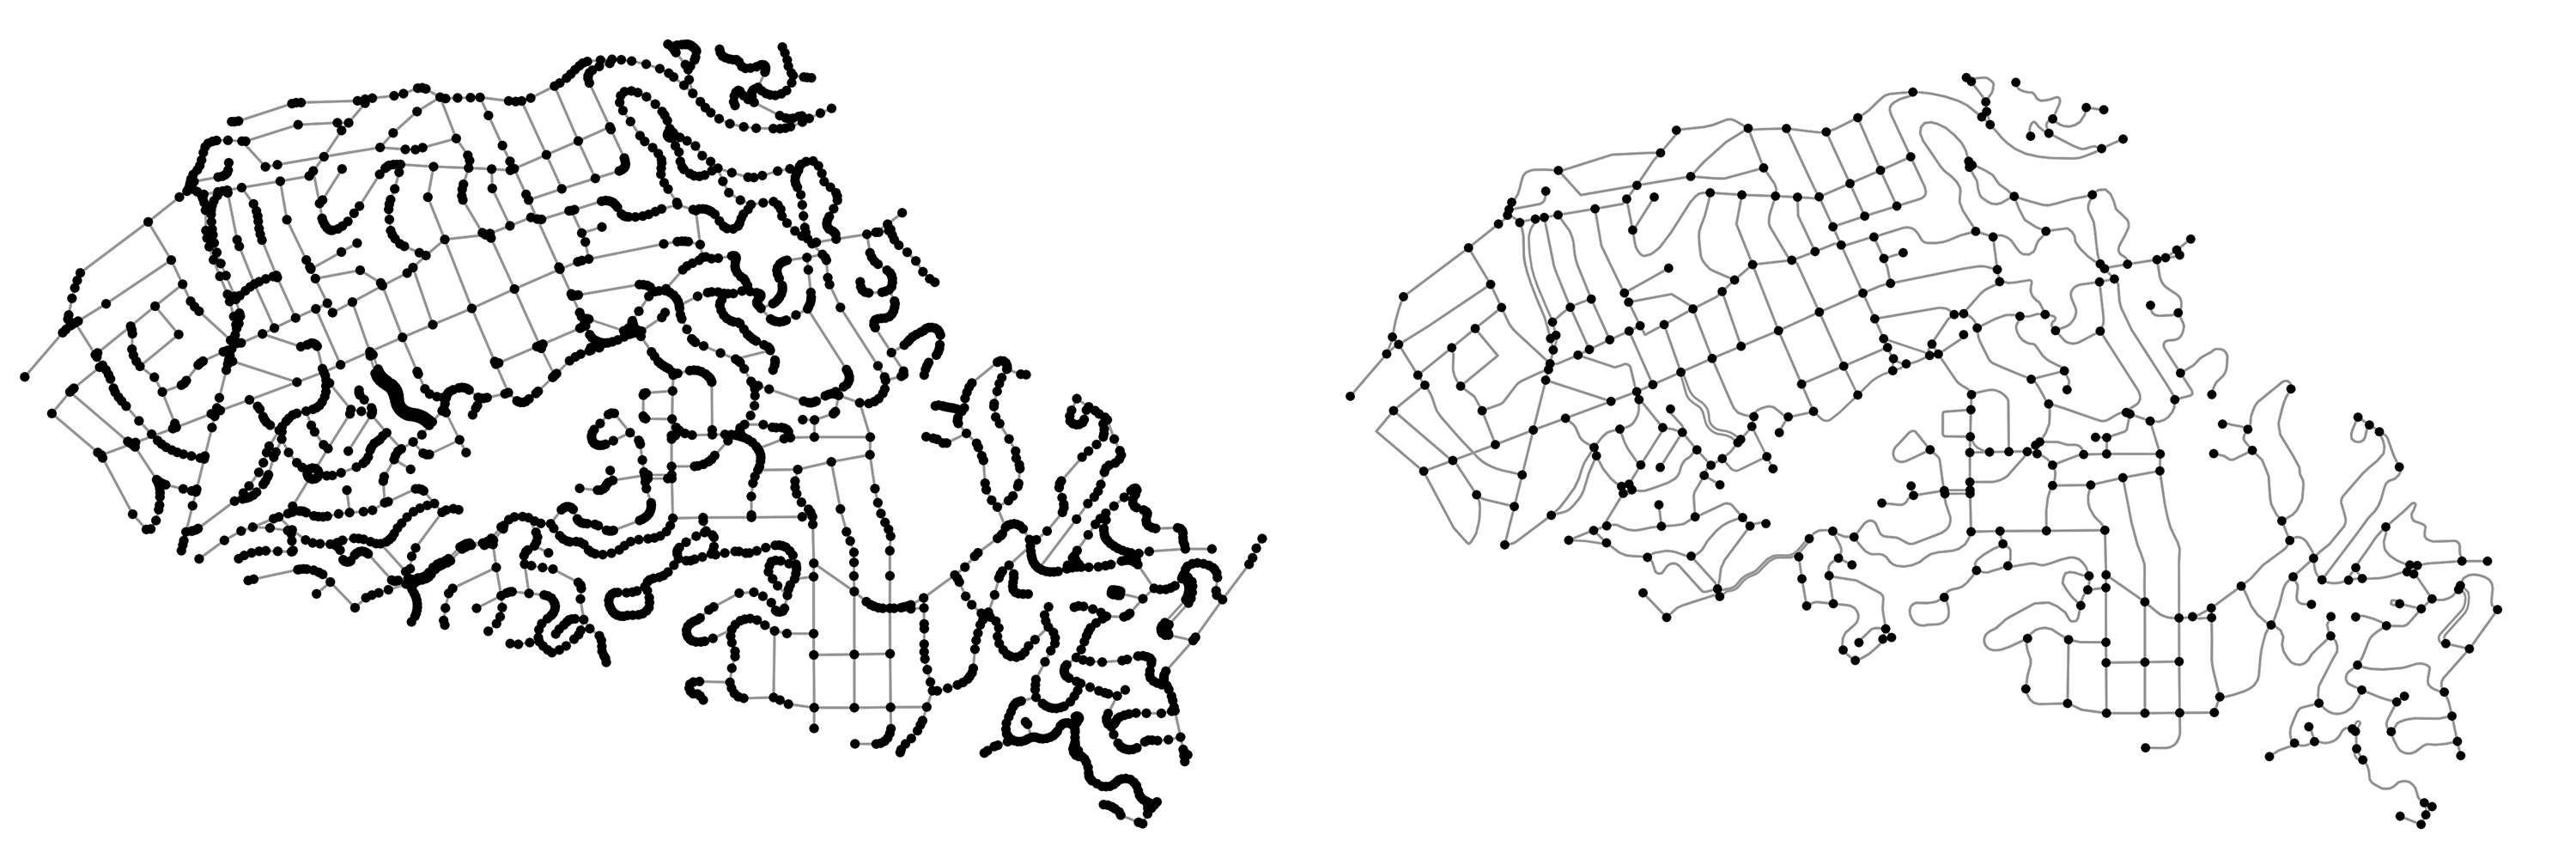
\includegraphics[width=\textwidth]
    {graphics/simplification_before_after.png}
    \caption{A suburban street network from OpenStreetMap data before OSMnx topology simplification (left) and after (right), with nodes in black and edges in gray. Note that the full spatial geometry is retained as edge metadata even though the edge itself is compressed to a single pair of origin and destination nodes.}
    \label{fig:simplification_before_after}
\end{figure}

We use OSMnx to download the road network for the nine-county San Francisco Bay Area. We use the 2016 US Census Bureau TIGER/Line shapefile of United States counties to define the spatial extents of these nine counties: Alameda, Contra Costa, Marin, Napa, San Francisco, San Mateo, Santa Clara, Solano, and Sonoma. We calculate a convex hull around these geometries to obtain a single polygon for the spatial query---this prevents the query from discarding any network elements that fall within our study area but outside of a county's borders (for example, bridges over the San Francisco Bay).

Next, we use OSMnx to download the drivable road network within this convex hull. OSMnx processes the detailed metadata tags to identify which paths are drivable. It then constructs them into a graph. This initial graph contains 1.2 million nodes and 2.3 million edges.

Next we filter the road network to retain only tertiary roads and larger. In OpenStreetMap terminology, the road types we retain comprise: motorway, motorway\textunderscore link, trunk, trunk\textunderscore link, primary, primary\textunderscore link, secondary, secondary\textunderscore link, tertiary, tertiary\textunderscore link, unclassified, and road. The \enquote{link} types are necessary to retain the connectors (such as on-ramps and off-ramps) between certain roads. The \enquote{road} type is standardly used in the OpenStreetMap community as a null value. The \enquote{unclassified} type technically refers to the British-style roads hierarchy, in which \enquote{unclassified} is the level below \enquote{tertiary} – that is, quaternary. However, it sometimes is used inconsistently in the United States, so we retain it for completeness.

\begin{figure}[htbp]
    \center
    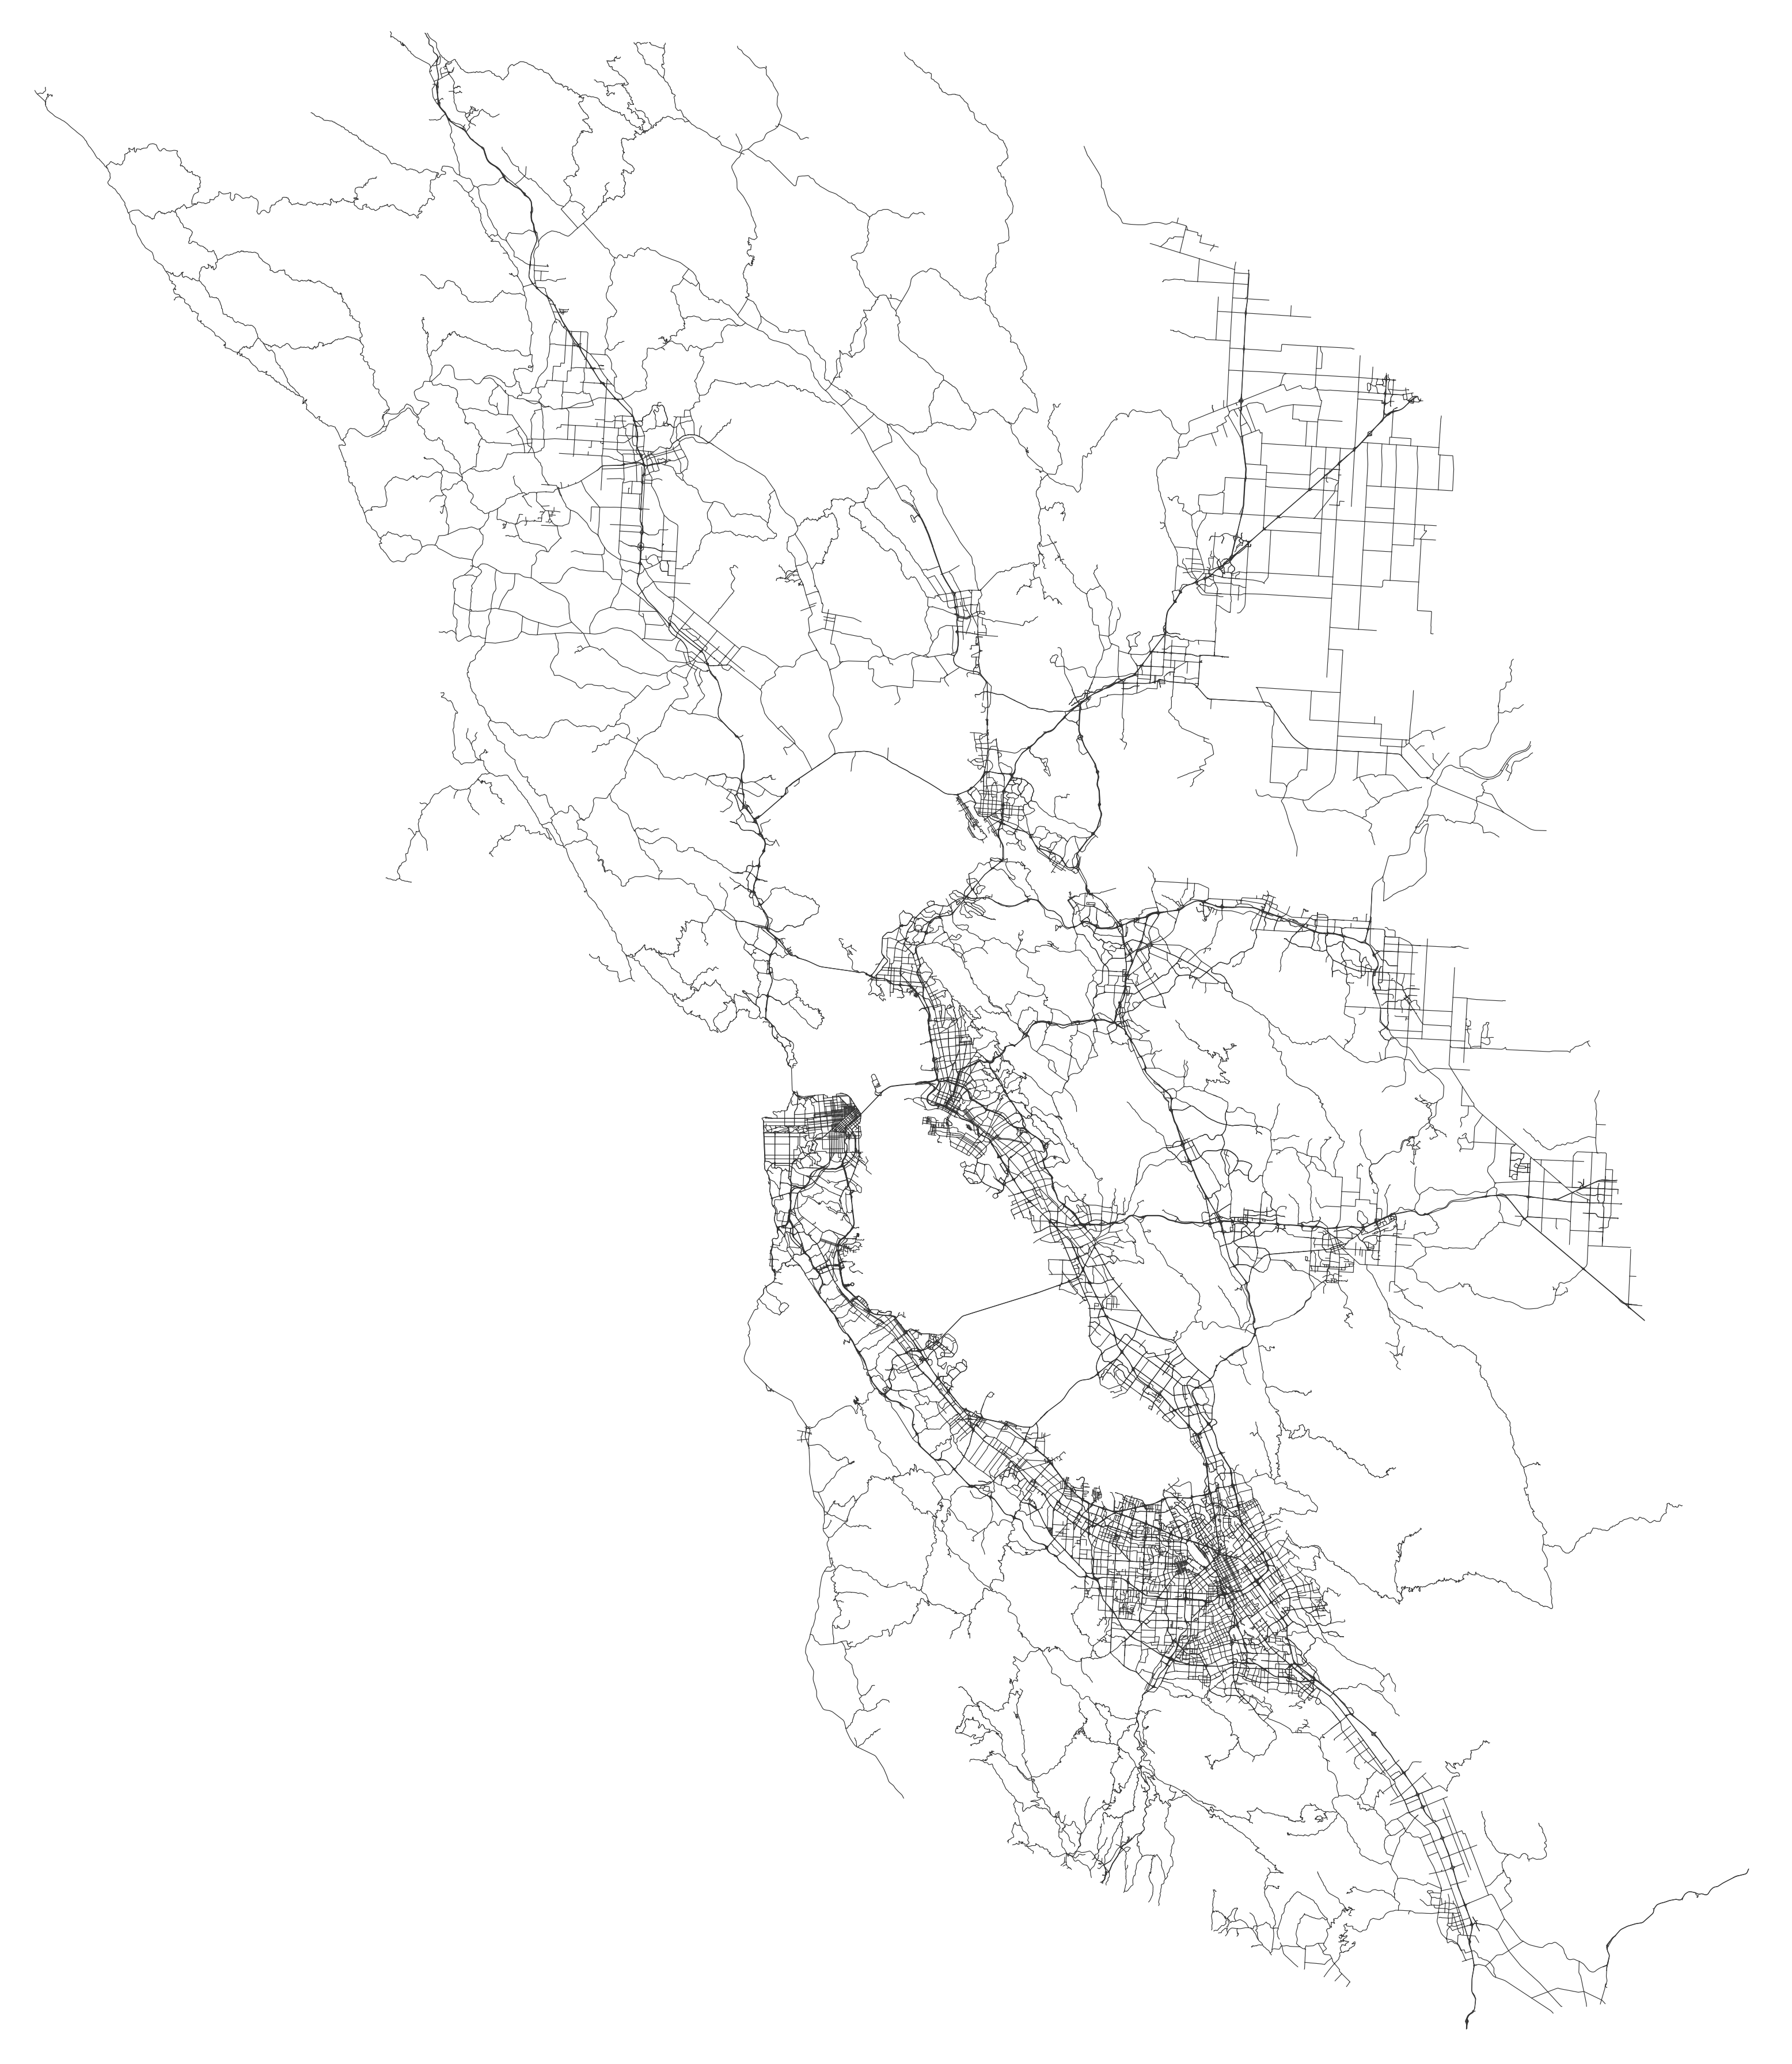
\includegraphics[width=\textwidth]
    {graphics/bay_area_network.png}
    \caption{The nine-county San Francisco Bay Area road network used in our modeling pipeline, created by OSMnx from OpenStreetMap data.}
    \label{fig:bay_area_road_network}
\end{figure}

After filtering out all edges not of these major types, we remove all isolated nodes then keep only the largest weakly-connected component of the graph. Finally, we simplify the graph using OSMnx then save it to disk as a GraphML file. GraphML is a standard, XML-based file format for storing and exchanging complete graph structure data. Our final graph contains 31,000 nodes and 66,000 directed edges representing 20,000 kilometers of roads across these 9 Bay Area counties, as seen in Figure \ref{fig:bay_area_road_network}.

\subsection{BPR coefficients calculation and assumptions}
To define the relationship between edge travel time and edge congestion we use the Bureau of Public Roads (BPR) congestion function. This BPR function has long been used by transportation engineers to model the increased time needed to traverse an edge when congestion is high. Once we have the final processed graph of the Bay Area road network, we calculate the BPR  curves' coefficients $a_0$, $a_1$, $a_2$, $a_3$, and $a_4$ for it. The BPR function is defined in Equation \ref{eq:bpr_function}.

\begin{equation}
    t_i = t^0_i (1 + \alpha (\frac{v_i}{c_i}) ^ \beta)
    \label{eq:bpr_function}
\end{equation}

where:

\begin{itemize}
    \item $t_i$ is the congested flow travel time on edge $i$
    \item $t^0_i$ is the free-flow travel time on edge $i$
    \item $v_i$ is the number of vehicles on edge $i$ per unit of time 
    \item $c_i$ is the capacity (i.e., maximum number of vehicles) of edge $i$ per unit of time
    \item $\alpha$ linearly increases the congested travel time with regards to the volume:capacity ratio
    \item $\beta$ exponentially increases the congested travel time with regards to the volume:capacity ratio
\end{itemize}

The $\alpha$ parameter was assigned a value of 0.15 in the original BPR curve, and the $\beta$ parameter was assigned a value of 4 in the original BPR curve. We adopt these default $\alpha$ and $\beta$ parameter values in this integrated modeling pipeline, but note that they are not the only way to parameterize this function. For instance, the TRB's NHCRP Report 716: Travel Demand Forecasting Parameters and Techniques provides various coefficients estimated using the 1985 Highway Capacity Manual \citep[p.~75]{transportation_research_board_highway_1985,transportation_research_board_travel_2012}.

Given this function, we further define the coefficients $a_0$, $a_1$, $a_2$, and $a_3$ as:
 
\begin{itemize}
    \item $a_0 = t0_i$, that is, the free-flow travel time
    \item $a_1$, $a_2$, and $a_3$ are always zero
\end{itemize}

Then we calculate the coefficient $a_4$ as defined by Equation \ref{eq:bpr_a4_coefficient}:

\begin{equation}
    a_4 = t^0_i \frac{\alpha}{c_i ^ {\beta}}
    \label{eq:bpr_a4_coefficient}
\end{equation}

To calculate these coefficients, we require per-edge data about capacity and free-flow travel time. To assemble these data, we require information about edge lengths, free-flow speed, and number of lanes. We use OSMnx to calculate these edge lengths. OpenStreetMap contains sparse data per-edge on maximum permitted speed and number of lanes. When these data are missing, we infer or impute them as per the defaults\footnote{The authors wish to thank Madeleine Sheehan and Alexander Skabardonis for providing some of these values.} in Tables \ref{table:free_flow_speed_defaults} and \ref{table:capacity_defaults}.

First, for each edge that is missing number of lanes data, we impute the value based on its edge type (which OpenStreetMap always provides as metadata). We calculate this imputed value by taking the median value of all edges of this type. Second, for each edge that is missing maximum permitted speed data, we infer the free-flow speed from a look-up table via edge type and number of lanes (see Table \ref{table:free_flow_speed_defaults}). We can now calculate free-flow travel time per edge as a function of free-flow speed and edge length, as defined in Equation \ref{eq:free_flow_travel_time}:

\begin{equation}
    t^0_i = \frac{d_i}{s_i}
    \label{eq:free_flow_travel_time}
\end{equation}

where:

\begin{itemize}
    \item $t^0_i$ represents free-flow travel time on edge $i$, in units of seconds
    \item $d_i$ represents the length of edge $i$, in units of meters
    \item $s_i$ represents free-flow speed (i.e. the maximum permitted speed of travel) on edge $i$, in units of meters per second
\end{itemize}

Next, we infer each edge's vehicle capacity (per lane per hour) from a look-up table via edge type and number of lanes (see Table \ref{table:capacity_defaults}). We then convert this capacity per lane per hour value to units of capacity per edge per second. Finally, we use these data to calculate the values of the $a0$ and $a4$ coefficients for the BPR curve. These calculations demand a caveat: due to missing data on OpenStreetMap, we are forced to infer or impute variables on many edges. Our assumptions on parameter values and capacity and speed limit defaults propagate through to our BPR coefficients.

\begin{table}[htbp]
\centering
\caption{Free-flow speed defaults by edge type and number of lanes, in units of miles per hour.}
\label{table:free_flow_speed_defaults}
\begin{tabular}{ l r r r r } 
    \hline
    Edge type & lanes=1 & lanes=2 & lanes=3 & lanes=4+ \\
    \hline
    motorway & 50 & 50 & 65 & 65 \\
    motorway\textunderscore link & 50 & 50 & 65 & 65 \\
    trunk & 45 & 45 & 45 & 45 \\
    trunk\textunderscore link & 45 & 45 & 45 & 45 \\
    primary & 30 & 30 & 30 & 30 \\
    primary\textunderscore link & 30 & 30 & 30 & 30 \\
    secondary & 25 & 25 & 25 & 25 \\
    secondary\textunderscore link & 25 & 25 & 25 & 25 \\
    tertiary & 20 & 20 & 20 & 20 \\
    tertiary\textunderscore link & 20 & 20 & 20 & 20 \\
    unclassified & 20 & 20 & 20 & 20 \\
    road & 30 & 30 & 30 & 30 \\
    \hline
\end{tabular}
\end{table}

\begin{table}[htbp]
\centering
\caption{Capacity defaults by edge type and number of lanes, in units of vehicles per lane per hour.}
\label{table:capacity_defaults}
\begin{tabular}{ l r r r r } 
    \hline
    Edge type & lanes=1 & lanes=2 & lanes=3 & lanes=4+ \\
    \hline
    motorway & 1900 & 2000 & 2000 & 2200 \\
    motorway\textunderscore link & 1900 & 2000 & 2000 & 2200 \\
    trunk & 1900 & 2000 & 2000 & 2000 \\
    trunk\textunderscore link & 1900 & 2000 & 2000 & 2000 \\
    primary & 1000 & 1000 & 1000 & 1000 \\
    primary\textunderscore link & 1000 & 1000 & 1000 & 1000 \\
    secondary & 900 & 900 & 900 & 900 \\
    secondary\textunderscore link & 900 & 900 & 900 & 900 \\
    tertiary & 900 & 900 & 900 & 900 \\
    tertiary\textunderscore link & 900 & 900 & 900 & 900 \\
    unclassified & 800 & 800 & 800 & 800 \\
    road & 900 & 900 & 900 & 900 \\
    \hline
\end{tabular}
\end{table}

\subsection{Linking zone-based travel demand to the network}

The ActivitySim component of our integrated modeling pipeline produces an output dataset of zone-to-zone travel demand data. To model this travel demand (and in turn traffic assignment) on our road network, we must convert the trip origins and destinations from zones to network nodes.

We use the shapefile of Traffic Analysis Zones (TAZs) from the Bay Area Metropolitan Transportation Commission (MTC) to acquire zone spatial extents. Then we calculate the centroid of each zone polygon. Finally, we identify the network node nearest to each zone's centroid by taking the minimum of a vectorized calculation of great-circle distances from the centroid to every node in the network, using the haversine formula defined in Equation \ref{eq:haversine_formula}:

 
\begin{equation}
    \delta_{gc} = r\cdot \arccos{(\sin{\Phi_1}\cdot\sin{\Phi_2} + \cos{\Phi_1}}\cdot\cos{\Phi_2}\cdot\cos{|\lambda_1 - \lambda_2|})
    \label{eq:haversine_formula}
\end{equation}

where:

\begin{itemize}
    \item $\delta_{gc}$ represents the great-circle distance between the two points, in meters
    \item $r$ represents the radius of the Earth, in meters
    \item $\Phi_1$ and $\Phi_2$ represent the geographical latitudes of the two points, in radians
    \item $\lambda_1$ and $\lambda_2$ represent the geographical longitudes of the two points, in radians
\end{itemize}

Now that we have the road network, its per-edge BPR coefficients, and node-based travel demand data, we are ready to model traffic assignment.
